\chapter{Introduction }

\section{Overview}
\subsection{Gravitational waves - a new window to the Universe}

Astrophysics overview - what could we see?  
\subsection{Core collapse supernovae} 
%
%%
\subsection{LIGO and Advanced LIGO} 
The LIGO interferometers are built to sense gravitational waves by measuring strain, or the change in length over the length of two 4km perpendicular arms. To accomplish this, a 1064~nm laser beam is split down each of the arms, reflected back via high reflectivity mirrors, and recombined. Any change in relative length between the arms will change the interference pattern for the recombined light, and we can infer the dynamics of the astrophysical source from the space-time perturbation manifested in this strain.

Searches for generic \gw{} transients, or \textit{bursts}, in data from previous LIGO science runs were able to make new and astrophysically meaningful upper limit statements (\cite{Vela}, \cite{BurstAllSky}, \cite{GRBs}), but their reach was limited by fundamental sources of noise, such as seismic, thermal, and shot noise as seen in Figure \ref{fig:iLIGO}.

\begin{figure} 
\centering
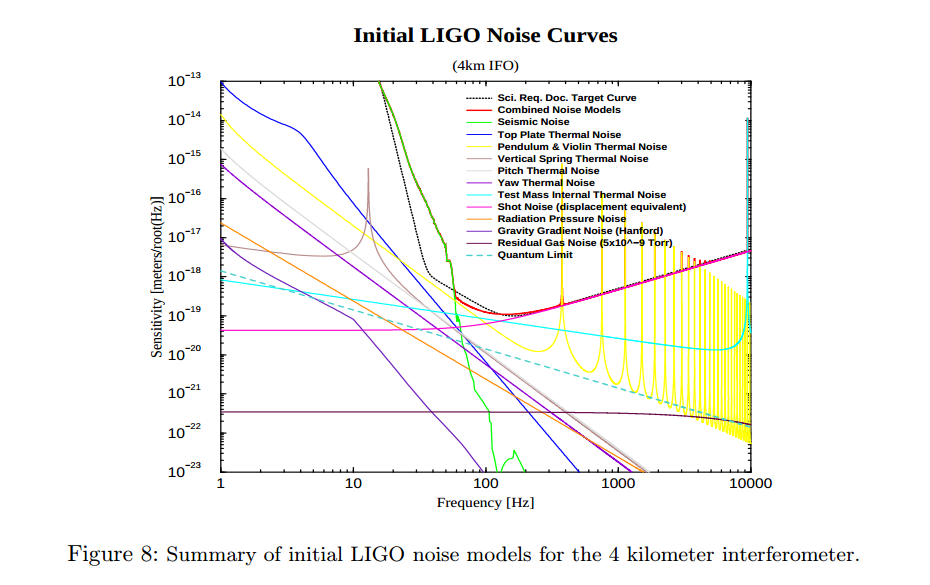
\includegraphics[width=\linewidth]{figures/iLIGO_noise_curve.png}
\caption{Fundamental sources of noise for iLIGO. Note the science requirement curve denoted with a dotted black line, the iLIGO combined noise curve in red, seismic noise in green limiting at lower frequencies, thermal noise in yellow limiting about 100Hz, and shot noise in magenta limiting at higher frequencies \cite{iLIGO_poster}.} 
\label{fig:iLIGO_noise}
\caption{Fundamental noise sources and their contribution to sensitivity in various frequency regimes.}
\label{fig:iLIGO} 
\end{figure}

\subsection{Extracting CCSN physics from Advanced LIGO data} 
\subsubsection{Detectability} 
\subsubsection{Waveform reconstruction}
extraction of rich, complex information

\subsection{Terrestrial sources of aLIGO noise and their impact on CCSN}
\subsection{Common sources of noise} 
\subsection{Transient noise}
\subsection{Seismic noise}
Seisveto paper - S6 DetChar 
\subsection{Terrestrial noise: impact on detectability, parameter estimation, and waveform reconstruction }
S6 all sky DQ 
NINJA2 results - glitches obscure parameter estimatio


%
%%
\section{General Relativity and Gravitational waves} 
\subsection{Prediction of gravitational waves} 
\subsection{Propagation of gravitational waves}
\subsection{Gravitational wave astronomy}

%
%%
\section{LIGO and Advanced LIGO}

 
\subsection{Advanced LIGO}

To combat noise sources that limited \gw{}  searches in previous science runs, the LIGO detectors are currently undergoing an instrumentation upgrade to Advanced LIGO, including the installation of active seismic isolation and improved suspensions systems for each mirror as well as improvements to the optics and laser subsystems \cite{Harry-aLIGO}. Advanced LIGO data will be usable for \gw{}  searches down to 10 Hz; a 30 Hz improvement over initial LIGO (compare Figures \ref{fig:iLIGO_noise} and \ref{fig:aLIGO_noise}). 

\begin{figure} 
\centering
\begin{subfigure}{.48\textwidth}
  \centering
  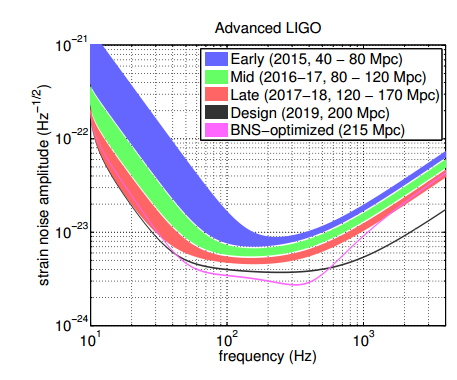
\includegraphics[width=\linewidth]{figures/aLIGO_noise_curve.png}
  \caption{The expected noise curves for different stages of Advanced LIGO science run data taking \cite{aLIGOoutlook}}. 
  \label{fig:aLIGO_noise}
\end{subfigure}%
\quad
\begin{subfigure}{.48\textwidth}
  \centering
  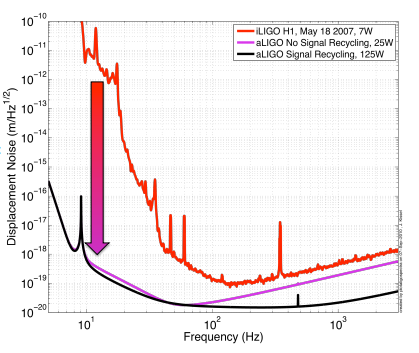
\includegraphics[width=\linewidth]{figures/aLIGO_performance_gain.png}
  \caption{The performance gained at 10Hz with new aLIGO seismic isolation instrumentation. \cite{KisselThesis}. Credit: J. Kissel.} 
  \label{fig:SEISUSgain}
\end{subfigure}
\caption{A comparison of anticipated Advanced LIGO noise curves, highlighting the improvement at low frequencies.}
\label{fig:aLIGO} 
\end{figure}

The Advanced LIGO detectors are quickly completing construction, installation, and testing and there could be a second generation interferometric \gw{} science run as soon as 2015 with Advanced Virgo following shortly after in 2016 (see Appendix for discussion of global interferometer network). The next two years are a key time to be exploring interesting potential \gw{}  sources and tuning our new instrumentation to optimize the potential for scientific discoveries. 

Characterization of the instrument before these science runs begin is crucial to making the first \gw{}  detection. The new Advanced LIGO instrumentation reduces seismic noise by six orders of magnitude at 10Hz and thermal noise by a factor of 10 around 100Hz (see Figure \ref{fig:SEISUSgain}). This brings Advanced LIGO closer to being a quantum limited detector, but introduces many new potential glitch mechanisms. 


\subsection{The LIGO interferometers and the global interferometer network}

There are two 4km LIGO interferometers - one in Livingston, Louisiana and one in Hanford, Washington. The hardware belonging to a third LIGO interferometer is in the process of being transferred to India. The 3km Virgo detector in Italy is also undergoing similar hardware upgrades to Advanced Virgo, the underground cryogenic detector KAGRA is being built in Japan, and the 600m GEO600 detector in Germany is testing new technology planned for future upgrades like light squeezing. Together, this network of advanced interferometers will increase sensitivity to gravitational waves tenfold and enable significantly improved sky localization \cite{Gonzalez-GWA}. 

\subsection{Advanced LIGO seismic isolation} 

Advanced LIGO features new complex instrumentation that needs to be carefully characterized: a 10-times more powerful laser, a new thermal compensation system, new suspensions, and an active seismic isolation. To prepare all subsystems, the detector characterization working group has appointed subsystem leads to direct characterization efforts for these subsystems and liaison with the commissioners and engineers. I have been serving as the seismic isolation subsystem lead for about a year and a half now, leading a team of a dozen researchers in projects aimed to better understand the seismic isolation performance and how it affects the \gw{} searches. 

It may seem nonintuitive that excess seismic noise, which limits the search range only at frequencies below 10 Hz, according to Figure \ref{fig:aLIGO_noise}, would be a candidate for interfering with transient \gw{}  searches above 40 Hz. However, local ground motion was one of the limiting noise sources in searches for transient \gw{}  sources during previous LIGO science runs (2005--2010). Seismic noise has been shown to couple with transient searches via an up-conversion mechanism (or mechanisms) that hasn't been well identified~\cite{Macleod-Seisveto}. 

For average motion, the Advanced LIGO active seismic isolation systems are designed to push the lower frequency bound of aLIGO sensitivity to the technological limit (see Figure \ref{fig:SEISUSgain} for a depiction of the improvements aLIGO is expected to achieve with this new instrumentation). 
The active seismic isolation systems are composed of several mechanically isolated platforms, known as stages - as seen in Figure \ref{fig:BSC_ISI}. To reduce seismic noise, the motion of each stage is measured with respect to the stage below it and controlled with precise, powerful actuators with a well-tuned feedback loop to remain as stationary as possible - as in Figure \ref{fig:SEI_iso} \cite{KisselThesis}. 

\begin{figure}[htb]
	\center{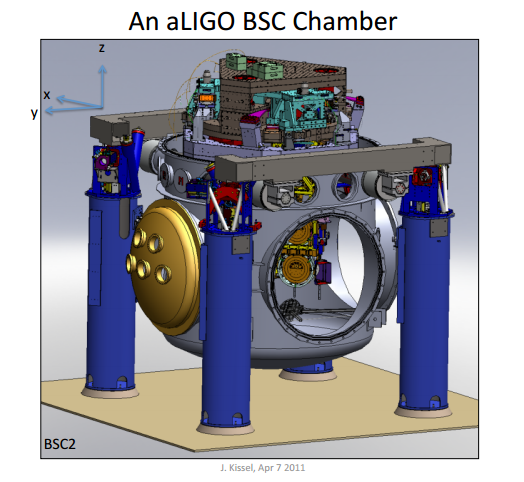
\includegraphics[scale=0.55]
	{figures/BSC_ISI.png}}
	\caption{\label{fig:BSC_ISI} A representation of the Advanced LIGO active isolation platforms and suspensions for the core optics. The Hydraulic External Pre-Isolator (HEPI) is in dark blue, the Internal Seismic Isolation (ISI) stages are in grey and teal at the top, and the quadruple suspension and optic can be partially seen through the representation of the circular opening. Credit: J. Kissel.}
\end{figure}

\begin{figure}[htb]
	\center{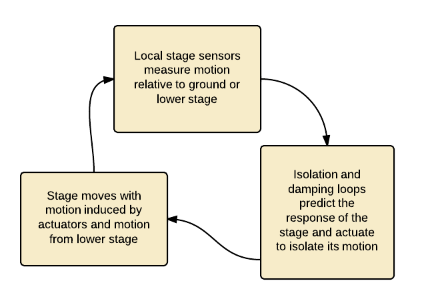
\includegraphics[scale=0.6]
	{figures/SEI_isolation_loop.png}}
	\caption{\label{fig:SEI_iso} This flowchart represents the basic feedback loop of the aLIGO active seismic isolation stages.}
\end{figure}

Advanced LIGO commissioners have demonstrated that the active seismic isolation systems so far installed perform very well in average motion during quiet seismic times - see Figure \ref{fig:HAM_ISI_current}.
However, a crucial unknown is how effectively the active seismic isolation systems mitigate transient seismic noise. Additionally, transient noise potentially introduced by the actuators themselves and how these may affect transient \gw{} searches has yet to be explored. 

\begin{figure}[htb]
\centering
\begin{subfigure}{.5\textwidth}
  \centering
  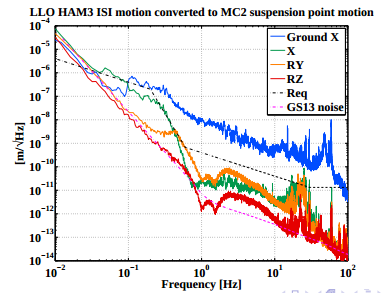
\includegraphics[width=\linewidth]{figures/Current_HAM_ISI_performance.png}
  \caption{Current HAM ISI performance spectra. Credit: R. DeRosa}
  \label{fig:HAM_ISI_current}
\end{subfigure}%
\begin{subfigure}{.5\textwidth}
  \centering
  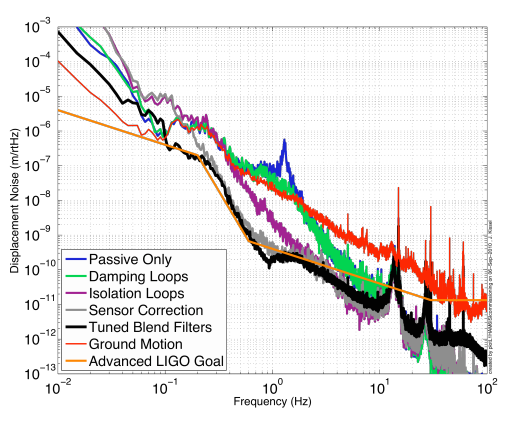
\includegraphics[width=\linewidth]{figures/SEI_SUS_spectra.png}
  \caption{aLIGO seismic noise requirements for core optics. Credit: J. Kissel.}
  \label{fig:SEISUS_spectra}
\end{subfigure}
\caption{On the left, a recent series of spectra showing the Internal Seismic Isolation (ISI) performance of an auxiliary optics chamber (known as 'HAM' or Horizontal Access Chamber'). The installed ISIs of core and auxiliary optics are currently performing better than aLIGO requirements at most frequencies in traditional average motion tests. 
On the right are spectra representing successive levels of isolation of core optic seismic isolation at design performance. Contributions from the quadruple suspensions are represented by 'Passive only'.}
\label{fig:test}
\end{figure}

\subsubsection{Suspensions}

The passive quadruple and triple suspensions provide significant seismic isolation at frequencies above 10Hz, as seen in Figure \ref{fig:SEISUS_spectra}. For active seismic isolation system characterization important to consider the active seismic isolation and suspension for each optic as complementary parts of a broader system with the same goal: to isolate the optics from local ground motion. There may sometimes be unexpected excess transient motion in the upper active isolation stages, but if this motion does not couple through the suspension masses to the motion of the optic, then it will not affect our search sensitivity. 




%%%%


